\chapter{Queueing Representation of Kinematic Waves}
\label{ch:kinematicwaves}
% ##################################################################################################################

\hfill \textbf{Author:} Gunnar Flötteröd

\begin{center} 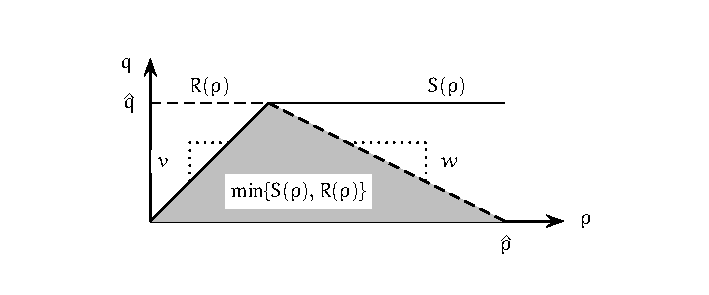
\includegraphics[width=0.4\textwidth, angle=0]{understanding/figures/waves/fig0.pdf} \end{center}

% ##################################################################################################################

\newcommand{\SINGLEQUEUESIM}{\gls{qsim}}
\newcommand{\DOUBLEQUEUESIM}{\gls{jdeqsim}}

\section{\label{sec:Introduction}Introduction}

\gls{matsim} comes with a number of \glspl{mobsim} (\cf
Sections~\ref{sec:using-mobsims},~\ref{sec:deqsim}), the most important ones
currently being the so-called \SINGLEQUEUESIM\ and the so-called
\DOUBLEQUEUESIM. These differ from the implementation perspective
(time-stepping vs.\ event-based, degree of parallelism), but they constitute
all (at least approximate) solvers of the same underlying traffic flow model.
The purpose of this chapter is to relate \gls{matsim}'s \glspl{mobsim} 
to the existing traffic flow theory. It should be acknowledged that there exist
similar simulation packages that are rooted in the same underlying modeling concepts 
\citep[][]{mahut-2007,zhou-2014}.

At the heart of \gls{matsim}'s traffic flow model is the flow-density relationship
(also called \gls{fd}) shown in Figure~\ref{fig:Fundamental-diagram}.
Given a long, homogeneous
road it predicts the average flow $q$ (in vehicles per time unit)
through any cross-section of that road, given an average vehicle density
$\varrho$ (in vehicles per length unit) on that road. 

% ----------
\createfigure%
{Fundamental diagram}%
{Fundamental diagram}%
{\label{fig:Fundamental-diagram}}%
{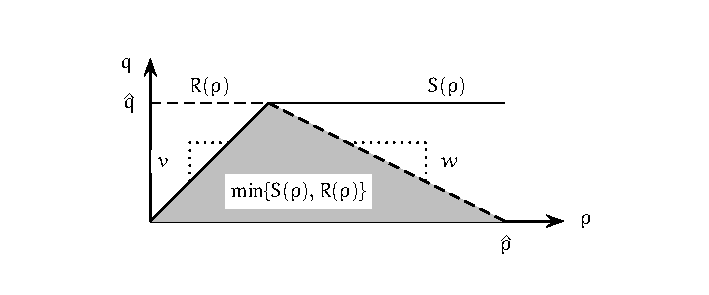
\includegraphics[width=0.99\textwidth, angle=0]{understanding/figures/waves/fig0.pdf}}%
{}
% ----------

The \gls{fd} is defined as the minimum of a sending function $S(\varrho)$
(solid) and a receiving function $R(\varrho)$ (dashed), resulting
overall in a triangular curve that is parametrized by the free flow speed $v$, 
the maximum density $\hat{\varrho}$ and the
backward shockwave speed $w$. The maximum velocity is an observable
parameter that can be set in the network file (\texttt{freespeed}
attribute of the \texttt{link} element). The maximum density equals
one over the length of a vehicle (\texttt{effectivecellsize} attribute
of the \texttt{links} element) for a single-lane link and needs to
be multiplied with the number of lanes (\texttt{permlanes} attribute
of the \texttt{link} element) otherwise. The backward wave speed turns
out to be the ratio of the length of a vehicle to the safety time
gap adopted by drivers in congested conditions. This parameter turns
out to be fairly constant; a vehicle length of 7.5\,meters and a time
gap of 2\,seconds leads to a value of 13.5\,kilometers per hour. 
The backward wave speed can be set in the \DOUBLEQUEUESIM\ through the
\lstinline|gapTravelSpeed| parameter; it currently cannot be set in the
\SINGLEQUEUESIM. \kaitodo{chk before going to print}
% \note{Can it be set somewhere, or is there a hardcoded value?} 
% \kai{QSim: Ist generell noch nicht implementiert, also auch nicht konfigurierbar.  
% Jdeqsim: Andreas, könntest Du das bitte mal nachschauen?}
% \ah{in \gls{jdeqsim} this can be configured by parameter \lstinline|gapTravelSpeed|. 
% Note: The default is there 15\,meters per second (not km/h). 
% Car size is configured with \gls{jdeqsim} parameter \lstinline|carSize| (default: 7.5\,meters).}

The considered \gls{fd} alone applies only in stationary conditions, where
it predicts that (i) flow increases linearly with density at low densities
(\ie in uncongested conditions); (ii) flow decreases linearly with
density at high densities (\ie in congested conditions); and (iii)
in-between it attains a maximal value that constitutes the flow capacity
\begin{eqnarray}
\hat{q} & = & \frac{vw\hat{\varrho}}{v+w}\label{eq:flow-cap}
\end{eqnarray}
 of the link. This parameter represents the maximum throughput of
the link in the absence of any other flow constraint (such as downstream
traffic lights or other bottlenecks), which are discussed further
below.

A realistic representation of non-stationary traffic flow (where density
and flow change over space and time) is possible by inserting the
\gls{fd} into a continuity equation (which intuitively models vehicle conservation,
in the sense that vehicles cannot vanish or spontaneously appear on
a road segment without on- and off-ramps). This leads to the \gls{kwm} 
of traffic flow \citep[][]{lighthill-1955,richards-1956},
where the sending and receiving function receive an intuitive interpretation:
The instantaneous flow across any interface, possibly with different
densities prevailing and \glspl{fd} applying up- and downstream of that interface,
is defined by (i) inserting the density upstream of the interface
into the upstream sending function, (ii) inserting the density downstream
of that interface into the downstream receiving function, and (iii)
taking the minimum of these two quantities \citep{Daganzo_TransResPartB_1994,lebacque-1996}.
Intuitively: The flow is limited by what can be sent from upstream
and what can be received downstream, but otherwise it is maximized.

The remainder of this chapter expresses \gls{matsim}\textquoteright{}s link
model (Section~\ref{sec:Link-model}) and its node model (Section~\ref{sec:Node-model})
in terms of the sending and receiving function framework of the \gls{kwm}.
Some technical detail is omitted from the presentation for the sake
of readability; pointers to the literature are provided.

% ##################################################################################################################
\section{\label{sec:Link-model}Link Model}
To compute the flows entering and leaving a link, one needs to know
how much flow can at most enter the link and how much flow can at
most leave the link. Both constraints depend on the internal (congestion)
state of the link. In symbols, one is interested in the instantaneous
receiving flow rate $R$ of the link's upstream end and the instantaneous
sending flow rate $S$ of the link's downstream end. Multiplying these
rates by the duration $\delta$ of a simulation time step then yields
the maximum number of vehicles that can enter respectively leave the link
during a time step.

\gls{matsim} also needs to compute these quantities. The way in which it
does so is rooted in Newell's {}''simplified theory of kinematic
waves'' \citep{newell-1993}, which provides a tracktable recipe for
computing the flow and the density anywhere inside of a link given
that one keeps track only of the flows at the link's up- and
downstream interface. In terms of the continuum model (\ie one that
allows for real-valued flows and densities at real-valued locations
and times) specified by \citet{newell-1993}, the cumulative in- and
outflow of a link are defined as
\begin{eqnarray}
N^{\text{in}}(t) & = & \int_{0}^{t}q^{\text{in}}(z)dz\label{eq:cum-in}\\
N^{\text{out}}(t) & = & \int_{0}^{t}q^{\text{out}}(z)dz\label{eq:cum-out}
\end{eqnarray}
where $t$ denotes time, $q^{\text{in}}$ and $q^{\text{out}}$are
the instantaneous in- and outflow rate (in vehicles per time unit)
of the link, and an initially (at $t=0$) empty link is assumed. From
\gls{matsim}'s vehicle-discrete perspective, the cumulative inflow (outflow)
at a given point in time hence represents the total number of vehicles
having entered (left) the link up to that point in time.

\citet{yperman-2006,yperman-phd} observe that if Newell's theory
allows to compute instantaneous densities anywhere in a link then
it also allows to compute densities at the up- and downstream end
of that link. Inserting these densities in the link's sending and
receiving function then allows to express sending and receiving flows
as functions of time-shifted cumulative in- and outflows only, with
the time-shifts being specified according to the original recipe of
\citet{newell-1993}:
\begin{eqnarray}
R(t) & = & \min\left\{ \hat{\varrho}L-\left[N^{\text{in}}(t)-N^{\text{out}}(t+\delta-L/|w|)\right],\,\hat{q}\delta\right\} \label{eq:R-yperman}\\
S(t) & = & \min\left\{ \left[N^{\text{in}}(t+\delta-L/v)-N^{\text{out}}(t)\right],\,\hat{q}\delta\right\} .\label{eq:S-yperman}
\end{eqnarray}
where $L$ is the length of the link and $\delta$ is the (small)
discrete time step length. \citet{yperman-phd} provides some 
intuition for this otherwise rather formal specification.

The connection to \gls{matsim} can now be made explicit by labeling the
two bracketed terms in \MyEqRef{eq:R-yperman} and \MyEqRef{eq:S-yperman}
as {}``upstream queue'' UQ and {}``downstream queue'' DQ \citep{osorio-2011a,osorio-2013b}:
\begin{eqnarray}
\text{UQ}(t) & = & N^{\text{in}}(t)-N^{\text{out}}(t+\delta-L/|w|)\label{eq:UQ-nonrek}\\
\text{DQ}(t) & = & N^{\text{in}}(0,t+\delta-L/v)-N^{\text{out}}(t)\label{eq:DQ-nonrek}.
\end{eqnarray}
These expressions can be given a recursive meaning. Evaluating
$\text{UQ}(t) - \text{UQ}(t - \delta)$ yields 
$[N^{\text{in}}(t) - N^{\text{in}}(t-\delta)] - [N^{\text{out}}(t+\delta-L/|w|) - N^{\text{out}}(t-L/|w|) ]$,
which under the assumption that flow rates are held constant throughout a simulation time step
simplifies into $\delta [ q^{\text{in}}(t-\delta) - q^{\text{out}}(t-L/|w|) ]$.
From this (and symmetric operations for DQ), one obtains
\begin{eqnarray}
\text{UQ}(t) & = & \text{UQ}(t-\delta)+\delta\left[q^{\text{in}}(t-\delta)-q^{\text{out}}(t-L/|w|)\right]\label{eq:UQ-rek}\\
\text{DQ}(t) & = & \text{DQ}(t-\delta)+\delta\left[q^{\text{in}}(t-L/v)-q^{\text{out}}(t-\delta)\right].\label{eq:DQ-rek}
\end{eqnarray}
These recursive definitions turn out to be the continuum version of
how the \DOUBLEQUEUESIM\ updates its link model: In
every time step, all vehicles that have just left the link are taken
out of the DQ and all vehicles that have entered the link $L/v$ time
units ago (corresponding to the free-flow travel time) are inserted
into the DQ. Similarly, all vehicles that have just entered the link
are put into the UQ and all vehicles that have left the link $L/|w|$
time units ago are only now taken out of the UQ. Further, inserting
(\ref{eq:UQ-nonrek}) and (\ref{eq:DQ-nonrek}) into (\ref{eq:R-yperman})
and (\ref{eq:S-yperman}) yields
\begin{eqnarray}
R(t) & = & \min\left\{ \hat{\varrho}L-\text{UQ}(t),\,\hat{q}\delta\right\} \label{eq:R-matsim}\\
S(t) & = & \min\left\{ \text{DQ}(t),\,\hat{q}\delta\right\} \label{eq:S-matsim}
\end{eqnarray}
which again corresponds to the way in which the \DOUBLEQUEUESIM\ 
evaluates the boundary conditions of a link: The amount of flow that
is allowed to enter the link is limited by the space in its UQ, and
the amount of flow that is allowed to leave the link is limited by the
number of vehicles in its DQ. 
% \note{Is this description compatible with the actual implementation?} 
% \kai{Das muss ich im Moment auf die jdeqsim beziehen, weil die QSim das ja noch gar nicht implementiert hat.  Bei der jdeqsim kenne ich mich aber nicht aus.  --  Aber das, was wir in der QSim derzeit probieren, sieht so aus.}

A \gls{mobsim} that implements the rules \MyEqRef{eq:UQ-rek}, \MyEqRef{eq:DQ-rek}
and \MyEqRef{eq:R-matsim}, \MyEqRef{eq:S-matsim} implements a \gls{kwm}-consistent
link model. This is almost the case for the \DOUBLEQUEUESIM,
which, in its implementation as of December 2014, has the sole deficiency
of not limiting the link's inflow to its flow capacity. 
% \note{Is this correct?} 
% \kai{Kenne mich mit jdeqsim nicht aus.  Man kann da irgendetwas einstellen.  Das, was wir in der QSim derzeit ausprobieren, wird keine link inflow capacity restriction haben.}
% \ah{in \gls{jdeqsim} there is \emph{no} maximum inflow capacity, there is only the \lstinline|minimumInFlowCapacity| parameter to prevent gridlocks.}
%
The \SINGLEQUEUESIM\ turns out to be a
particular instance of the same model where the backward wave speed
is set to $\left|w\right|=L/\delta$. Inserting this into \MyEqRef{eq:UQ-rek}
leads to
\begin{eqnarray}
\text{UQ}(t) & = & \text{UQ}(t-\delta)+\delta\left[q^{\text{in}}(t-\delta)-q^{\text{out}}(t-\delta)\right],
\end{eqnarray}
which represents nothing but the total number of vehicles in the link.
This corresponds indeed to the behavior of the \SINGLEQUEUESIM,
where the inflow to a link is limited only by the available space
in the link as a whole. Letting $\left|w\right|=L/\delta$ means that
the \SINGLEQUEUESIM\ behaves like a \gls{kwm} with an extremely
high backward shockwave speed, which physically means that a queue
on the link does not dissolve from its downstream end but moves {}''en
block'' over the link. 

% ##################################################################################################################
\section{\label{sec:Node-model}Node Model}
All \glspl{mobsim} in \gls{matsim} implement the same node model. Somewhat surprisingly,
this node model can be traced back at least to \cite[][under the name of ``fair intersections'']{CetinBurriNagel2003queue}, whereas
the literature based on which its consistency with the \gls{kwm} can be
established is only a few years old \citep{tampere-2010b,floetteroed-2011a,corthout-2012}. 

Nodes in \gls{matsim} have no spatial dimension; they merely connect up-
and downstream links. \citet{tampere-2010b} specify a set of requirements
for a (continuum) node model to be consistent with the \gls{kwm}. They require
that the flow through the node shall be maximized subject to the following
constraints:
\begin{enumerate}
\item Flows are non-negative and conserved within the node. This means that
vehicles cannot drive backwards, and they must neither disappear nor
spontaneously appear within the node.
\item Flow ratios comply with exogenous specified turning fractions. For
instance, if it is specified that 20\,\% of the outflow of link
$i$ shall turn into link $j$, then the amount of flow that actually
advances from link $i$ into link $j$ shall indeed be 20\,\%
of the flow that actually leaves link $i$.
\item Sending flows of upstream links and receiving flows of downstream
downstream are not exceeded. The meaning of this is explained in Section~\ref{sec:Link-model}.
\item The invariance principle of \citet{lebacque-2005} is satisfied. The
intuitively most important implication of this principle is that the
advancement of a queuing vehicle is not affected by the vehicles
behind it.
\item A {}``supply constraint interaction rule'' is satisfied. It defines
how the limited receiving flow of a downstream link is shared
by competing upstream link. In practical terms, a right-of-way specification.
\end{enumerate}
\citet{floetteroed-2011a} specify an {}``incremental node model''
that satisfies these requirements, and they also provide an intuitive
and computationally efficient solution algorithm. In each simulation
time step, this algorithm incrementally (hence the name) moves flow
from upstream links into downstream links. It does so such that all
of the aforementioned constraints are satisfied anytime during the
transfer, and it terminates only once no more flow can be moved. In
consequence, the ultimately moved flows also comply with all constraints,
and they are maximal. 

Now consider the code documentation of \gls{matsim}'s \lstinline|queuesim.QueueNode.moveNode|
(as of December 2014):
\begin{quote}
\noindent \texttt{Moves vehicles from the inlinks' buffer to the outlinks
where possible. The inLinks are randomly chosen, and for each link
all vehicles in the buffer are moved to their desired outLink as long
as there is space. If the front most vehicle in a buffer cannot move
across the node because there is no free space on its destination
link, the work on this inLink is finished and the next inLink's buffer
is handled.}
\end{quote}
This is an informal description of how the incremental node model
of \citet{floetteroed-2011a} works, given that one adopts the conventions
that the sending flow of a link is stored in its {}``buffer'' and
that the receiving flow of a link is labeled here as the free space
in (the upstream queue of) that link. A more detailed inspection of
the underlying implementation also does not reveal any inconsistencies
with the incremental node model specification.

There are two aspects of the \gls{matsim} node model that is not reflected
by the above code comment.
\begin{itemize}\styleItemize
\item The sending flows of an upstream link may be limited by by an outflow
capacity that is below the flow capacity \MyEqRef{eq:flow-cap} of
that link, for instance to approximate the capacity reduction resulting
from a downstream traffic light. This is still consistent with the
framework described above.
\item The selection probability of {}``inLinks'' is proportional to their
flow capacity, meaning that links with higher capacity send on average
more flow. This is again consistent with \citet{floetteroed-2011a}
and constitutes a concrete {}``supply constraint interaction rule'',
as required by \citet{tampere-2010b}.
\end{itemize}
The relative simplicity of \gls{matsim}'s intersection logic may be refined
in many regards; for instance, turning pockets may be added and conflicts
within the intersection may be modeled (\cf Chapter~\ref{ch:signalslanes}). 
%\note{I think Dominik has done something like this. Need to find a reference.} \kai{Andreas: Das wäre die ''lanes core extension''.}\ah{gracias}
However, some caution is needed when implementing such extensions.
The present node model is, due to its simplicity, guaranteed to yield
unique node flows. This property needs to be revisited when turning
to more complicated specifications \citep{corthout-2012}.

% ##################################################################################################################
\section{\label{sec:kinematicwaves-summary}Summary}
This chapter demonstrated that \gls{matsim}'s mobility simulation is already
very close to implementing a particle-discretized instance of the
\gls{kwm}. For full consistency, one needs to (i) use the \DOUBLEQUEUESIM\ 
(or to implement a realistic backward wave speed in the \SINGLEQUEUESIM)
and to (ii) limit the inflow of a link by its flow capacity (which
corresponds to the maximum of its triangular \gls{fd}). 
%\note{Is this correct? Or is there already ``full consistency'' with the KWM?.}
%%\kai{Folgend einige Sätze von AH, die eingearbeitet oder verworfen werden müssten.  M.E.\ interessant vor allem im Hinblick auf MFD.}
% 
% \ah{
% \gls{jdeqsim} (Section~\ref{sec:using-jdeqsim}) is the double-queue \gls{mobsim}, which is \emph{not} the default \gls{mobsim}.
% 
% \gls{qsim} (Section~\ref{sec:using-qsim}) is the single-queue \gls{mobsim}, currently extended as shown in research avenues in Section~\ref{sec:researchavenues-double-queue-mobsim}.
% }

% ##################################################################################################################

% Local Variables:
% mode: latex
% mode: reftex
% mode: visual-line
% TeX-master: "../main"
% comment-padding: 1
% fill-column: 9999
% End: 
